\chapter{Introduction}\label{chap:1}

As a theory of elementary particles and their interactions, the Standard Model of particle physics (SM) is both extremely impressive and notably incomplete. While capable of extremely precise predictions, which have been extensively verified by experimental observation, it does not account for a number of phenomena such as dark matter, dark energy, particle mass differences, gravity, and the abundance of matter over antimatter in the universe. These omissions in the theory must ultimately be resolved with the discovery of new physics beyond the SM (BSM). 

Searches for new physics employ various strategies: some looking for evidence of exotic processes or particles by use of high energy colliders or low background experiments, and others relying on high precision measurements of SM predicted parameters, looking for evidence of new physics at the point where theory and experiment diverge.

The Fermilab Muon $g-2$ experiment (E989) takes the latter approach, aiming to measure the anomalous magnetic moment of the muon, $a_{\mu}$, to a precision of 140 parts-per-billion (ppb). At the time of writing, the combination of first result for $a_{\mu}$ from E989 \cite{SummaryRun1}, with a precision of 460 ppb, and the final result of previous iteration of the Muon $g-2$ experiment at Brookhaven National Laboratory (BNL E821) \cite{BNLFinalReport} presents $4.2\sigma$ tension with the SM \cite{aMuSM}. If the discrepancy persists beyond $5\sigma$, and if no inaccuracies are discovered in the theoretical calculation of $a_{\mu}$, then new physics will be required to explain the anomaly. Additionally, E989 will conduct a world-leading search for the electric dipole moment (EDM) of the muon, $d_{\mu}$, projecting to improve on the current experimental upper limit of $|d_{\mu}|<1.8\times10^{-19}$ $e\cdot$cm, set by E821 \cite{BNLEDM}, by at least an order of magnitude. While the SM predicts a muon EDM of $\mathcal{O}(10^{-36})$ $e\cdot$cm\footnote{This estimate is based on the upper limit for the electron EDM \cite{ImprovedElectronEDMLimit}, and is discussed further in Chapter \ref{chap:1} Section \ref{sec:TheEDM}.}, which is far beyond the reach of current experimental sensitivity, a large muon EDM is allowed by certain well-motivated extensions to the SM; some of which can simultaneously accommodate the observed discrepancy in $a_{\mu}$. If a muon EDM is discovered at E989, it would signal a BSM source of combined charge conjugation and parity (CP) violation in the lepton sector, which may be critical in explaining the matter-antimatter asymmetry of the universe.

This thesis will focus on efforts towards a muon EDM search at E989. In this introductory chapter, the theory of lepton dipole moments will be outlined and the muon EDM search will be motivated in the context of new physics models. Chapter \ref{chap:2} will introduce the essential physics principles of the experiment, while Chapter \ref{chap:3} will discuss the specific techniques and hardware that comprise E989. Chapter \ref{chap:4} will detail the development and execution of a novel technique for measuring the radial component of the E989 storage ring magnetic field to a precision of $<1$ parts-per-million (ppm). This work ensures that the radial magnetic field, which can mimic an EDM signal, does not present a limiting source of systematic uncertainty in search for $d_{\mu}$ in Run-1, and beyond. Chapter \ref{chap:5} describes the large-scale simulation efforts which are essential to the characterisation of sources of systematic uncertainty in the measurement, and, critically, the momentum dependent dilution of the EDM signal. In Chapter \ref{chap:6}, a blinded search for $d_{\mu}$ in Run-1 using data from straw tracker detectors is presented, including an assessment of sources of systematic uncertainty, which is concluded with an estimation of a preliminary upper limit on $|d_{\mu}|$. Finally, Chapter \ref{chap:7} concludes this thesis, providing a summary of results and discussion as to the outlook of the search for a muon EDM at Fermilab. 

\section{The anomalous magnetic moment of the muon, $a_{\mu}$} \label{sec:TheMDM}
%
The magnetic dipole moment, $\vec{\mu}$, of a subatomic particle with mass $m$, charge $e$, and spin $\vec{s}$ is described by the expression %\footnote{Natural units, where $\hbar=c=1$, will be assumed throughout this thesis, unless stated otherwise.} 
%
\begin{equation} 
  \vec{\mu} = g\left(\frac{Qe}{2m}\right)\vec{s},
  \label{eqn:MDM}
\end{equation}
%
where $Q=\pm1$. $g$ is the $g$-factor: a dimensionless quantity which characterises the strength of the coupling between the magnetic moment and the spin. Classically, where the spin angular momentum may be compared to the total orbital angular momentum of a rotating distribution of charges, the $g$-factor would be equal to one \cite{Jackson}. For particles on the subatomic scale, however, it has been extensively proven that $g\neq1$. %By describing the behaviour of the magnetic moment in an external magnetic field, $\vec{B}$, in terms of the interaction Hamiltonian 
%
% \begin{equation} 
%   \mathcal{H} = -\vec{\mu}\cdot\vec{B}, 
%   \label{eqn:TotalHamiltonian1}
% \end{equation}
% %
% which is may be understood as the potential energy of the system, allowed  experimentalists were able to deduce through hyperfine
The origin of this deviation arises in part from relativistic effects, which may be reconciled with quantum mechanics via the Dirac equation: giving the prediction that $g=2$ for spin 1/2 particles (fermions). While this prediction holds at leading order, the interaction between the fermion and an external magnetic field includes contributions to the $g$-factor from higher order virtual particle loop diagrams at the fermion-photon vertex, known as radiative corrections, so that $g\neq2$. In the case of the electron and the muon, $g$ is slightly greater than 2. This deviation is the anomalous magnetic moment, $a$, which is defined as 
%
 % relativistic quantum field theories such as QED and the SM require the inclusion of the effects from higher order processes, commonly known as radiative corrections. 
%
\begin{equation}
  a = \frac{g-2}{2},
  \label{eqn:AnaMagMom}
\end{equation}
% 
allowing Equation \ref{eqn:MDM} to rewritten in the form
%
\begin{equation}
  \vec{\mu} = (1+a)\frac{e\hbar}{2m},
  \label{eqn:MDM2}
\end{equation}
% 
separating the magnetic moment into two parts: the Dirac moment and the \textit{anomaly} (the Pauli moment) \cite{LeptonDipoleMoments}. 

\begin{figure}[b!]
\centering{}
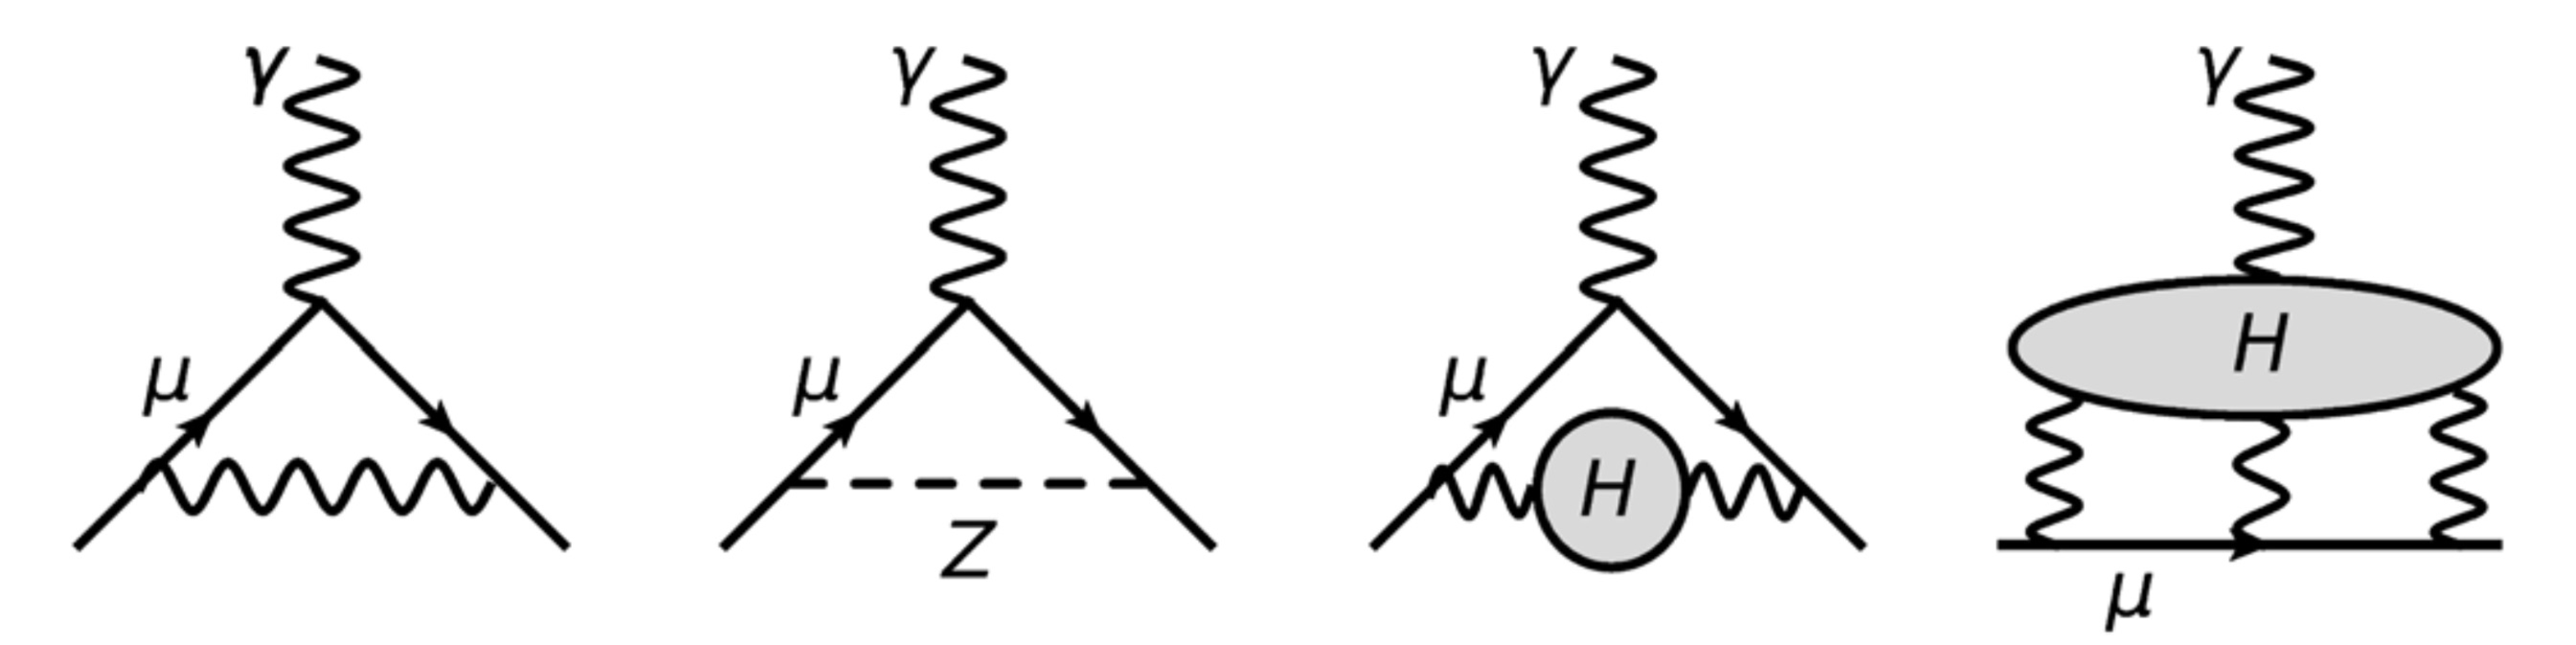
\includegraphics[trim={0 0 0 0},clip,width=0.89\textwidth]{Images/Chapter1/FeynmanDiagrams.pdf}
\caption{SM contributions to $a_{\mu}$. From left to right: leading order QED (Swinger), leading order electroweak, hadronic vacuum polarisation, and hadronic light-by-light scattering. Image reproduced from \cite{SummaryRun1}.}
\label{fig:SMContributions}
\end{figure}

The anomalous magnetic moment of the electron, $a_{e}$, was first measured by Kusch and Foley in 1947 \cite{KuschAndFoley}, with the leading order quantum electrodynamics (QED) radiative correction being famously calculated by Swinger soon after \cite{Swinger}. Since then, $a_{e}$ has become the most precisely predicted \cite{ElectronAnomalyPrediction} and measured \cite{ElectronAnomalyMeasurement} physical quantity ever: a stringent test of QED and a resounding success for the SM.

The anomalous magnetic moment of the muon, $a_{\mu}$, while not as suitable for probing QED as the electron, presents a far more promising avenue in the search for new physics \cite{TheMuonAnomalyAndNewPhysics}. Quantitatively, the reason for this is that a particle with mass $M$, where $M>>m$ (with $m$ being the elementary fermion mass), makes a contribution to the anomaly $a$ on the scale of 
%
\begin{equation}
  \delta a \sim C\cdot\left(\frac{m}{M}\right)^{2}, 
  \label{eqn:NewPhysicsScale}
\end{equation}
%
where $C=\delta m/m$, $\delta m$ being the new physics contribution to the fermion mass, which is highly dependent on the details of the new physics model in question (discussed further in Chapter \ref{chap:1} Section \ref{sec:NewPhysics}). Given that the muon is $\sim200$ times more massive than the electron, this implies that the muon magnetic anomaly is $\sim4\times10^{4}$ times more sensitive to the higher mass-energy scales where BSM physics is most likely to reside.
%
\begin{figure}[t!]
\centering{}
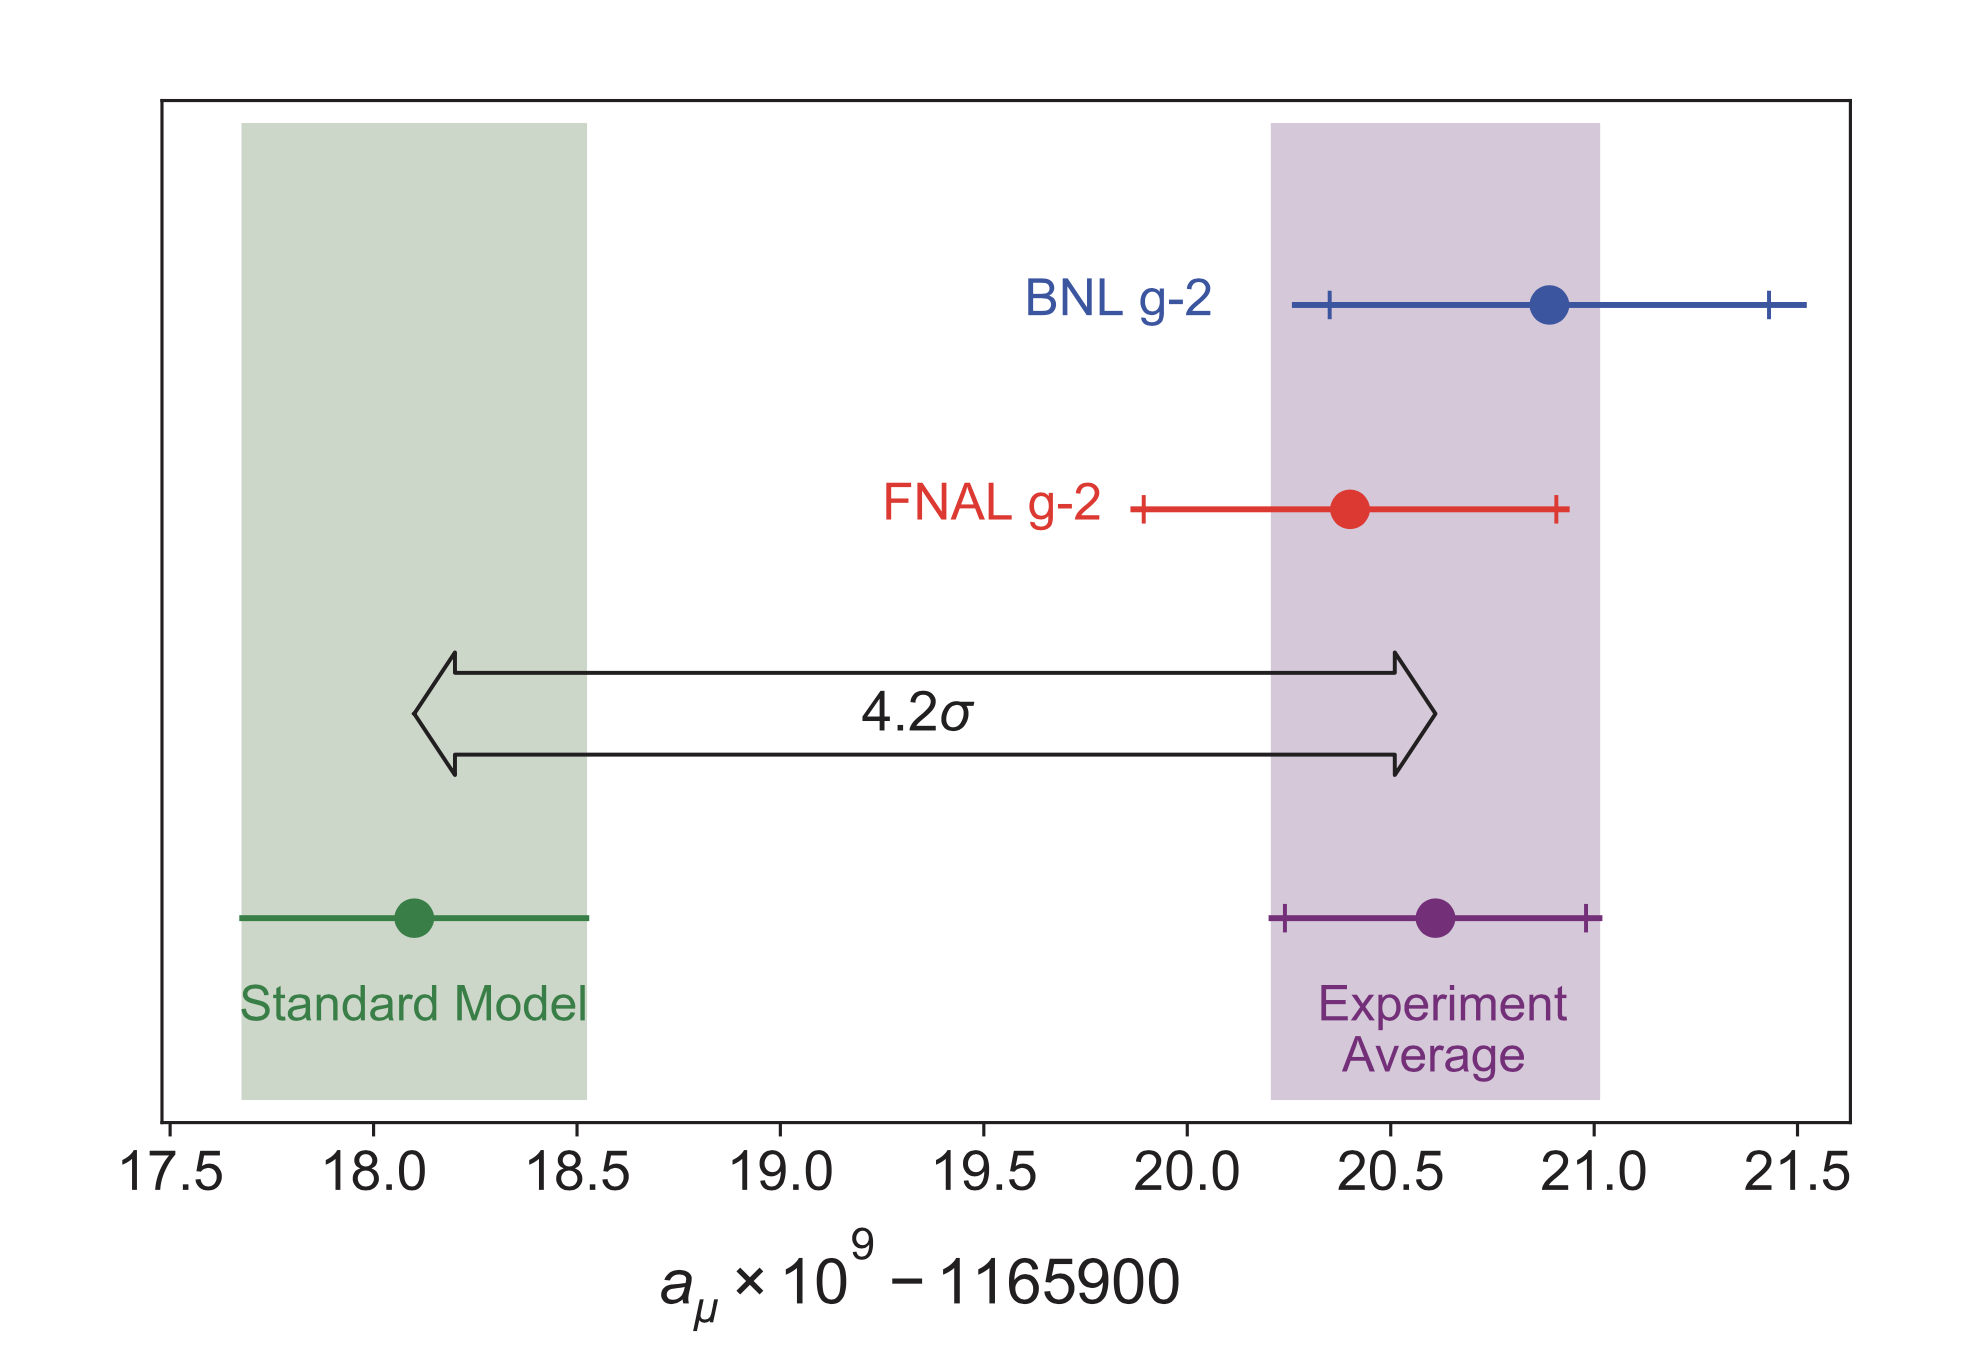
\includegraphics[trim={0 0 0 0},clip,width=0.89\textwidth]{Images/Chapter1/ResultPlotRun1.png}
\caption{Current experimental values of $a_{\mu}$ from Brookhaven E821 and Fermilab E989, as well as the experimental average, compared with the SM prediction. Image reproduced from \cite{SummaryRun1}.}
\label{fig:Run1Result}
\end{figure}
%

Within the SM, $a_{\mu}$ is composed of contributions from all sectors: the electromagnetic (QED), electroweak (EW), and hadronic (had), so that 
%
\begin{equation}
  a_{\mu}^{\text{SM}} = a_{\mu}^{\text{QED}} + a_{\mu}^{\text{EW}} + a_{\mu}^{\text{had}}, % \,( +\, a_{\mu}^{\text{BSM}}), 
  \label{eqn:SMContributions}
\end{equation}
%
where Feynman diagrams summarising the classes of SM contributions to $a_{\mu}$ are shown in Figure \ref{fig:SMContributions}. If there exists a discrepancy between experiment and the SM, $\Delta a_{\mu} = a_{\mu}^{\text{Exp}} - a_{\mu}^{\text{SM}}$, then a fourth (BSM) contribution must included, so that 
%
\begin{equation}
  a_{\mu}^{\text{Exp}} = a_{\mu}^{\text{SM}} + a_{\mu}^{\text{BSM}}. % \,( +\, a_{\mu}^{\text{BSM}}), 
  \label{eqn:AllContributions}
\end{equation}
%
At present, the SM prediction for the muon magnetic anomaly is $a_{\mu}^{\text{SM}}=(116591810\pm43)\times10^{-11}$ \cite{aMuSM}, while the current combined experimental value, which includes input from the first result from Fermilab E989 \cite{SummaryRun1} and the final result from Brookhaven E821 \cite{BNLFinalReport}, is $a_{\mu}^{\text{Exp}}=(116592061\pm41)\times10^{-11}$; so that the discrepancy stands at $\Delta a_{\mu} =(251\pm59)\times10^{-11}$. As illustrated in Figure \ref{fig:Run1Result}, this presents a $4.2\sigma$ tension between theory and experiment which, while not yet conclusive, indicates that new physics extensions to the SM may be required to account for the anomaly. The topic of new physics is expanded upon in Section \ref{sec:NewPhysics}.% Moreover, since E989 has yet to fold the vast majority of its total dataset into the measurement, the discrepancy is set to exceed the 5$\sigma$ threshold for discovery in the near future.
%

\section{The electric dipole moment of the muon, $d_{\mu}$} \label{sec:TheEDM}

In addition to a magnetic dipole moment, Dirac's theory predicts that subatomic particles may also possess an electric dipole moment (EDM), $\vec{d}$ \cite{LeptonDipoleMoments}. Classically, an EDM is a measure of the permanent polarisation of a system of electric charges. For the simplest case of two opposing point charges, $\pm q$, separated by a distance $\vec{r}$, the EDM is given by $\vec{d}=q\vec{r}$. More generally, $\vec{d}$ is equal to the integral of the charge density, $\rho(\vec{r})$, over the charge volume, so that
%
\begin{equation} 
  \vec{d} = \int{\vec{r}\rho(\vec{r})\,d^{3}r},
  \label{eqn:EDMIntegral}
\end{equation}
%
where $\vec{r}$ has it's origin at the centre of charge distribution \cite{Jackson}. In the case of elementary fermions, which are treated as point-particles of no spatial extent within the SM, the classical argument would follow that such particles must have a EDM of zero. In quantum mechanics, however, a non-vanishing EDM is allowed by polarisation of the vacuum field around the particle. Like the magnetic moment, the EDM must be directed along the spin vector, the only vector-like property associated with an elementary particle, and is expressed in form similar to Equation \ref{eqn:MDM}:
%
\begin{equation} 
  \vec{d} = \eta \left(\frac{Qe}{2mc}\right)\vec{s},
  \label{eqn:EDM}
\end{equation}
%
where $c$ is the speed of light in a vacuum. $\eta$ is a dimensionless quantity, analogous to the magnetic $g$-factor, which describes the strength of the coupling between the EDM and the spin. $\eta$ may be expressed in terms of fundamental constants, so that
%
\begin{equation} 
  \eta = \frac{4dmc}{Qe\hbar},
  \label{eqn:eta}
\end{equation}
%
where $d$ assumes the convention
%
\begin{equation} 
  \vec{d} = d\cdot\hat{s}. %= d\cdot\frac{\hbar}{2} %\frac{\vec{s}}{|\vec{s}|}.
  \label{eqn:scalarEDM}
\end{equation}
%dsvds 

Unlike its magnetic counterpart, the EDM of the muon and other subatomic particles breaks the symmetries parity, $P$, where $(t,x)\rightarrow(t,-x)$, and time reversal, $T$, where $(t,x)\rightarrow(-t,x)$. This $P$ and $T$ symmetry breaking arises from the differing properties of axial vectors and polar vectors under $P$ and $T$ transformations \cite{LeptonDipoleMoments}. Axial vectors, which describe a rotation about an axis, are even under $P$ (they do not change sign) and polar vectors are odd. Magnetic field vectors, $\vec{B}$, are axial and electric field vectors, $\vec{E}$, are polar. Spin is an axial vector, making the dipole moments $\vec{\mu}$ and $\vec{d}$ axial vectors by Equations \ref{eqn:MDM} and \ref{eqn:EDM}. The third symmetry is charge conjugation, $C$, where $q\rightarrow-q$, under which all quantities mentioned here are odd. The combined symmetry $CPT$ is expected to hold, so it follows that if $\vec{B}$ is even under $P$ then it must be odd under $T$. The same logic applies for $\vec{E}$ and $\vec{s}$. The various transformation properties of $\vec{E}$, $\vec{B}$, $\vec{\mu}$, and $\vec{d}$, are given in Table \ref{tbl:CPT}. 

\begin{table}[h!]
\centering
\begin{tabular}{l|ccc}
\hline
\hline
 & $\vec{E}\quad$ & $\vec{B}\quad$ & $\vec{\mu}$ or $\vec{d}\quad$ \\ 
\hline
 $C\quad$ & $-\quad$ & $-\quad$ & $-\quad$ \\ 
 $P\quad$ & $-\quad$ & $+\quad$ & $+\quad$ \\
 $T\quad$ & $+\quad$ & $-\quad$ & $-\quad$ \\
\hline
\hline
\end{tabular}
\caption{The transformation properties of $\vec{E}$, $\vec{B}$, $\vec{\mu}$, and $\vec{d}$.}
\label{tbl:CPT}
\end{table}

The external magnetic and electric fields, $\vec{B}$ and $\vec{E}$ may be related to their corresponding dipole moments by the interaction Hamiltonian
%
\begin{equation} 
  \mathcal{H} = -\vec{\mu}\cdot\vec{B}-\vec{d}\cdot\vec{E}, 
  \label{eqn:TotalHamiltonian1}
\end{equation}
%
from which it can be deduced that the magnetic part of the interaction is $CP$ even and the electric part, the EDM, is $CP$ odd. This means that subatomic particle EDMs violate $CP$ symmetry: one part of Sakharov's criteria \cite{Sakharov} for a universe dominated by matter rather than antimatter. 

Clearly, particle EDMs provide a unique insight into fundamental physics, and have been considered as such since Purcell and Ramsey first proposed a search for the neutron EDM as a means of testing P symmetry in 1950 \cite{PurcellAndRamsey}. Since then, however, no permanent EDM has been observed for any particle or atom \cite{ChuppEDMReview}. Moreover, the SM predictions for the magnitude of particle EDMs are vanishingly small, well below their current upper limits and out of reach of today's experiments. This is demonstrated Table \ref{tbl:ParticleEDMs}, where the upper limits for the EDM of the proton, neutron, electron, and muon are presented; along with their SM predicted values and corresponding references. 

\begin{table}[t!]
\centering
\begin{tabular}{l|ccc}
\hline
\hline
 Particle & EDM upper limit [$e\cdot$cm] & SM prediction [$e\cdot$cm] & References \\ 
\hline
 Proton & $2.0\times10^{-26}$ (95\% C.L.) & $\mathcal{O}(10^{-32})$ & \cite{199HgEDMLimits}, \cite{ProtonNeutronEDMPred}  \\ 
 Neutron & $1.6\times10^{-26}$ (95\% C.L.) & $\mathcal{O}(10^{-32})$ &  \cite{199HgEDMLimits}, \cite{ProtonNeutronEDMPred}  \\
Electron & $1.1\times10^{-29}$ (90\% C.L.) & $\mathcal{O}(10^{-38})$ & \cite{ImprovedElectronEDMLimit}, \cite{ElectronEDMPred} \\
 Muon & $1.8\times10^{-19}$ (95\% C.L.) & $\mathcal{O}(10^{-36})$ & \cite{BNLEDM}, \cite{ElectronEDMPred} \\
\hline
\hline
\end{tabular}
\caption{The upper limits for the EDM of the proton, neutron, electron, and muon, along with their SM predicted values and corresponding references.}
\label{tbl:ParticleEDMs}
\end{table}


% \myworries{Mention Purcell and Ramsey \cite{PurcellAndRamsey}.} If a non-zero muon EDM is discovered at Fermilab it would provide the first evidence of $CP$ violation in the lepton sector. Additional sources of $CP$ violation in the SM, such as that arising from a non-zero muon EDM, are highly sought after since levels of proven $CP$ violation in the SM, arising from the hadron sector\footnote{\myworries{$K^{0}\rightarrow\pi^{+}\pi^{-}$ and B-mesons. This is an area where I really do not know what I'm talking about but it should really be discussed. In any case it's likely to come up in a viva. Need some references.}}, are insufficient to account for the matter-antimatter asymmetry of the universe.

The SM prediction for the magnitude of the muon EDM in Table \ref{tbl:ParticleEDMs} is estimated based on the electron EDM upper limit, under the assumption of minimal flavour violation (MFV) \cite{MFV} which requires that EDMs scale linearly with mass across generations of leptons, as follows
%
\begin{equation}
  d_{\mu} \approx d_{e}\frac{m_{\mu}}{m_{e}}.
  \label{eqn:EDMMassScaling}
\end{equation}
%
If this assumption holds, then the muon EDM is inaccessible by current experiments, and will remain so for the foreseeable future. However, MFV scaling is called into question by the observation of flavour anomalies in $B$-decays, such as the recent result from the LHCb experiment \cite{LHCb2021}, lending support to SM extensions which could allow for a muon EDM within reach of E989. Further discussion on this topic is given in the following section. 

% The current upper limit on the muon EDM was set by the BNL Muon $g-2$ experiment, at $|d_{\mu}|<1.8\times10^{-19}$ $e\cdot$cm \cite{BNLEDM}. The Fermilab Muon $g-2$ experiment, with a substantially reduced statistical uncertainty and various improvements to experimental hardware, aims to improve upon this limit by at least an order of magnitude\footnote{\myworries{This estimate seems to vary depending on who you ask. We must have a proper idea of what we can do with our projected stats.}}. 

% \clearpage

\section{New physics}\label{sec:NewPhysics}

% There are numerous `new physics' extensions to the SM which could account for discrepancy $\Delta a_{\mu}$, or allow for a large muon EDM, or both, in some scenarios. This section will provide a brief overview of this topic.

The discovery of a large muon EDM would signal a significant departure from the SM. In particular, it would necessitate a BSM model involving a new complex parameter with a large CP violating phase, far in excess of that allowed within the SM. It would also indicate a breakdown of the linear mass scaling of EDMs between lepton generations, making it incompatible with the assumption of MFV. 

The discrepancy $\Delta a_{\mu}$ and the bounds on a muon EDM in BSM models are related: the effective field Hamiltonian for the $g-2$ interaction involves a complex Wilson coefficient, $c_{R}^{\mu\mu}$, which has a real part relating to the magnetic anomaly and an imaginary part to a non-vanishing EDM. In the various scenarios which resolve $\Delta a_{\mu}$ with the introduction of heavy TeV-scale particles, the parameter $C$ in Equation \ref{eqn:NewPhysicsScale} must be enhanced by allowing the chirality flip of the muon\footnote{In quantum field theory, the operator corresponding to $a_{\mu}$ connects left- and right-handed muons, making $g-2$ a chirality flipping interaction.} to be provided by a new massive fermion. This so-called chiral enhancement automatically introduces an unconstrained CP violating phase in the imaginary part of $c_{R}^{\mu\mu}$, allowing for a large muon EDM. Contours of $|d_{\mu}|$ as a function of the Wilson coefficient phase and $\Delta a_{\mu}$ are shown in Figure \ref{fig:WilsonCoeff} \cite{CombinedExplantionsForaMuAndEDM2018} \cite{CombinedExplantionsForaMuAndEDM2020}, with red bands indicating $\Delta a_{\mu}$ preferred from experiment\footnote{Excluding the most recent result from Fermilab \cite{SummaryRun1}.}, a dark blue band indicating the projected sensitivity of the Fermilab muon EDM search, and a light blue indicating the same for a proposed search experiment at PSI \cite{PSI}. From this, it may be inferred that a muon EDM may be measurable at Fermilab, assuming a contribution to $\Delta a_{\mu}$ from BSM models with chiral enhancement.

\begin{figure}[t!]
\centering{}
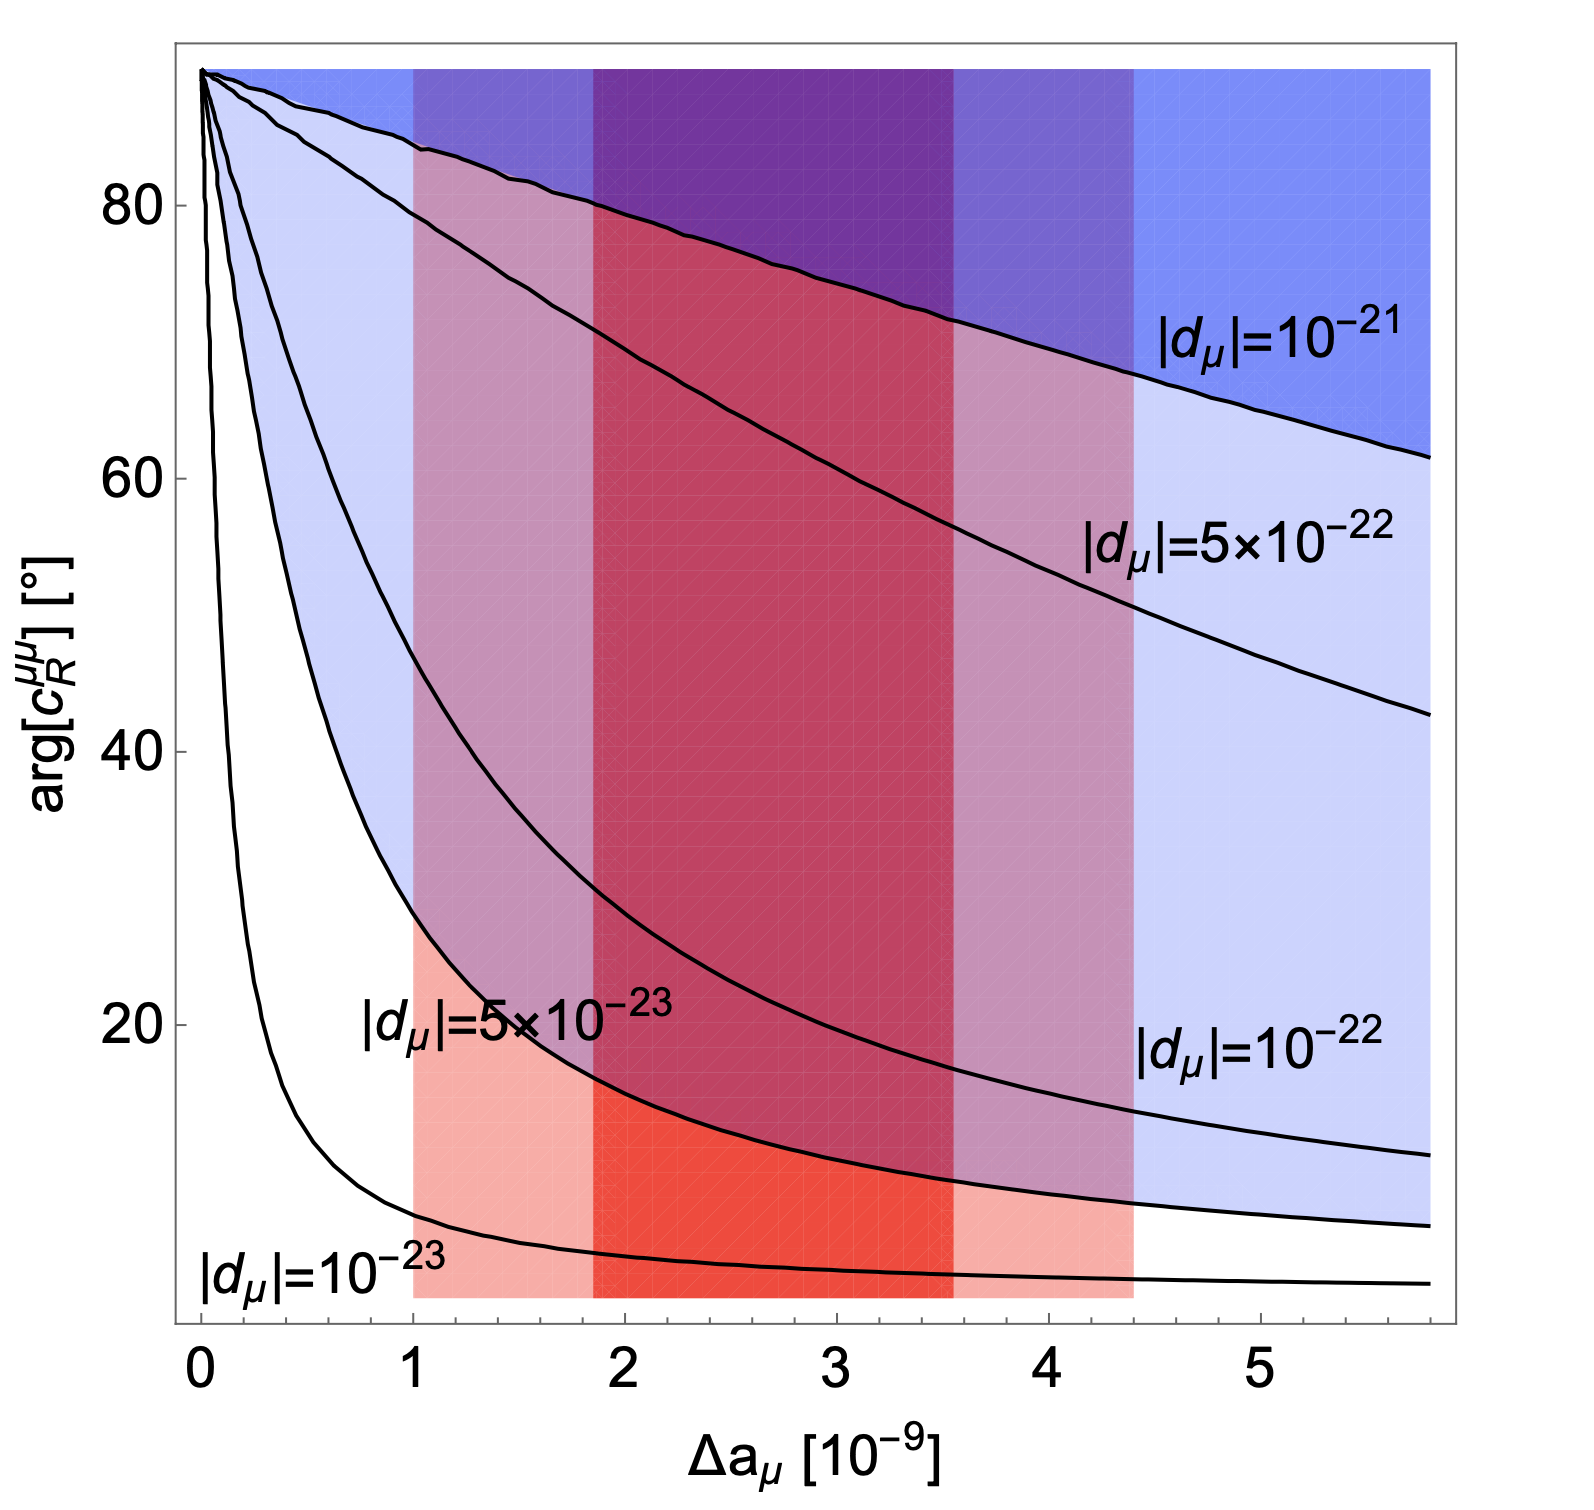
\includegraphics[trim={0 0 0 0},clip,width=0.69\textwidth]{Images/Chapter1/WilsonCoeff.png}
\caption{Contours of $|d_{\mu}|$ as a function of the Wilson coefficient phase and $\Delta a_{\mu}$. The red bands indicating $\Delta a_{\mu}$ preferred from experiment (which does not include the most recent Fermilab result \cite{SummaryRun1}), the dark blue band indicating the projected sensitivity of the Fermilab muon EDM search, and the light blue indicating the sensitivity of a proposed experiment at PSI \cite{PSI}. Image reproduced from \cite{CombinedExplantionsForaMuAndEDM2018}.}
\label{fig:WilsonCoeff}
\end{figure}

A well-known example of a model which can both provide chiral enhancement and accommodate $\Delta a_{\mu}$, and violate MFV scaling, is the minimally supersymmetric SM (MSSM). Supersymmetry (SUSY) involves the introduction of so-called superpartners to SM particles, which have values of spin offset by $1/2$ from their SM counterparts, so that SM fermions have a bosonic superpartner and vice versa. In the MSSM, chiral enhancement is provided by the parameter $\tan\beta$, which is the ratio of vacuum expectation values of the two Higgs fields in the model. MSSM parameter space capable of resolving $\Delta a_{\mu}$ has been severely constrained by the persistent lack of evidence from the LHC and dark matter searches, with scenarios involving smuons and heavy charginos requiring unfavourably large values of $\tan\beta$. However, one scenario which could accommodate the discrepancy involves a Bino-like\footnote{The $B$-boson superpartner.} lightest supersymmetric particle (LSP) and slepton loop contribution, allowing for a wide range of mass scales and $\tan \beta$ values \cite{NewPhysicsExplanations2021}. 

A concrete alternative to the MSSM are models which introduce heavy scalar leptoquarks (LQ): BSM bosons which couple simultaneously to SM leptons and quarks, carrying both lepton and baryon number. Scalar LQ models are minimally single particle extensions to the SM, and can resolve $\Delta a_{\mu}$ via virtual loop interactions at the muon-photon vertex with a chiral enhancement factor of $m_{t}/m_{\mu}$, where $m_{t}$ is the top quark mass \cite{NewPhysicsExplanations2021}. While many LQ models have been excluded, they remain well-motivated by both $\Delta a_{\mu}$ and the aforementioned flavour anomalies which also call MFV into question.

All considered, the muon EDM search at Fermilab is well motivated by the current landscape of new physics models, some of which allow for measurable values of $d_{\mu}$ while simultaneously accommodating the discrepancy $\Delta a_{\mu}$. The discussion presented here is far from exhaustive, and further reading on this topic may be found in \cite{CombinedExplantionsForaMuAndEDM2018}, \cite{CombinedExplantionsForaMuAndEDM2020}, and \cite{NewPhysicsExplanations2021}.


% Additional models which involve chiral enhancement 

% Searches at the LHC, such as at the CMS experiment \cite{CMS_2018}, indicate LQ masses in excess of 1 TeV. 



% LQ searches at the LHC place constraints from B decays. Many LQ models have been excluded, only S1 and R2 models are OK. Fine tuning means that only ones just above the. 



% with a chiral enhancement factor of $m_{t}/m_{\mu}$, 
% complex Wilson coefficient of the effective Hamiltonian relates to former and the imaginary part to the latter.


%The discrepancy $\Delta a_{\mu}$ may be interpreted as an indirect indication of new physics, meaning new physics can only be discovered by the construction of a model which both resolves the discrepancy and produces predictions that may be verified in other experiments. In contrast, 

% sectors, since the electron Such extensions are well motivated however, and can predict elementary particle EDMs with far exceed those predicted in the SM. A concrete example of such a model is 


%  which is far beyond that expected 


% New physics models which resolve $\Delta a_{\mu}$  

% For models involving radiative fermion mass generation, where fermion masses are radiatively induced from loops involving new physics, C is $\mathcal{O}({1})$ \cite{TheMuonAnomalyAndNewPhysics}. 

% As introduced in the previous section, the factor $C=\delta m_{\mu} / m_{\mu}$ in Equation \ref{eqn:NewPhysicsScale}, which defines the mass-energy scale of new physics contributions to $a_{\mu}$, is highly model dependent. In the case of models involving an expansion of the local $SU(3)\times SU(2) \times U(1)$ symmetry of SM to a larger gauge group, with the inclusion of additional gauge bosons $Z^{\prime}$ and $W^{\prime}$ which could , $C$ is found to be $\mathcal{O}(\alpha/4\pi)$ ($\alpha$ being the fine-structure constant). In this case, the scale of new physics would be very low -- on the order of the $Z$-boson mass -- which is difficult to reconcile with the lack of evidence for such physics from collider experiments. The same is true for models which invoke extra dimensions \cite{TheMuonAnomalyAndNewPhysics} \cite{StockingerChapter}.

% That said, light new physics may still resolve $\Delta a_{\mu}$, provided that the coupling is small enough that new physics remains hidden from experimental observation. One popular of class of models of this type are those which involve the addition of a hidden $U(1)$ symmetry to the SM, with a corresponding gauge boson called the dark photon. The dark photon can interact with the muon via kinetic mixing with the SM photon, with the dominant contribution to $\Delta a_{\mu}$ being proportional to the kinetic mixing parameter $\epsilon$. However, the current measured value of $a_{e}$ \cite{ElectronAnomalyMeasurement} constrains the dark photon mass to a range of 20-500 MeV, which is then excluded by various dark photon search experiments \myworries{Give one example}. That said, extensions to dark photon models which involve additional kinetic mixing with the $Z$-boson, so-called `dark Z' models, may still be viable for masses below 1 GeV, although they remain tightly constrained \cite[and references therein]{NewPhysicsExplanations2021}.

% Alternatively, new physics solutions for $\Delta a_{\mu}$ may be realised at higher mass scales, which requires a mechanism to enhance $C$. This is typically related to the muon chirality flip in the $g-2$ interaction\footnote{In quantum field theory, the operator corresponding to $a_{\mu}$ connects left- and right-handed muons.}, which may be provided by a new heavy particle. This so-called chiral enhancement is a feature of various BSM models. For example, those involving the introduction of supersymmetric (SUSY) particles, so-called superpartners of SM particles, with their spin differing from their SM counterparts by $1/2$, so that SM fermions have a bosonic superpartner and vice versa. These superpartners could participate in the virtual loop interactions at the muon-photon vertex and modify $a_{\mu}$. In the minimally supersymmetric SM (MSSM), chiral enhancement is provided by the parameter $\tan\beta$, which is the ratio of vacuum expectation values of the two Higgs fields in the model. MSSM parameter space capable of resolving $\Delta a_{\mu}$ has been severely constrained by the persistent lack of evidence from the LHC and dark matter searches, with scenarios involving smuons and heavy charginos requiring unfavourably large values of $\tan\beta$. One scenario which could accommodate the discrepancy involves a Bino-like\footnote{The $B$-boson superpartner.} lightest supersymmetric particle (LSP) and slepton loop contribution, allowing for a wide range of mass scales and $\tan \beta$ values 

% \cite{NewPhysicsExplanations2021}. 

% Minimal leptoquark models involve the addition of one new particle to the SM. 



% Regarding the muon EDM, a model which invokes chiral enhancement is highly relevant to the EDM. 

% $a_{\mu}$ is related to $d_{\mu}$ because the real part of complex Wilson coefficient of the effective Hamiltonian relates to former and the imaginary part to the latter. In BSM scenarios which invoke chiral enhancement of $C$, the phase of imaginary part may be unconstrained, meaning that the $d_{\mu}$ may be very large. Models which allow for a large EDM must also involve scaling which does 

% A key feature of both of these extensions is a scaling with lepton generation rather than lepton mass. This is particularly relevant, since searches for a muon EDM provide a unique opportunity to search for EDMs in a second generation particle 



% In general, a model which 

% \myworries{2HDM relates to the higgs.}. Leptoquark models 

% %two-Higgs-doublet models (2HDM), and leptoquark (LQ) models, which will be discussed in turn. SUSY particles are the 


% The scale of new physics, defined by Equation \ref{eqn:NewPhysicsScale}, may be enhanced or suppressed by an additional factor $C$, which is highly dependant on the details of the new physics model in question. 



% This section will provide a brief overview of this topic.% drawing from discussion given in , \cite{TheMuonAnomalyAndNewPhysics}, , and ... %Many of these models have already been tightly constrained the by measurements of $a_{\mu}$ and $d_{\mu}$ already undertaken, and 



% Another class of BSM models are those which involve the introduction of supersymmetric (SUSY) particles,  These SUSY particles are the so-called superpartners of SM particles, with their spin differing from their SM counterparts by $1/2$, so that SM fermions have a bosonic superpartner and vice versa. SUSY models are appealing because they can enhance $C$ by a factor of $\tan\beta$ (often referred to as chiral enhancement), which is the ratio of vacuum expectation values of the two Higgs fields. The dominant SUSY contributions to $a_{\mu}$ typically involve loop corrections from sleptons, neutralinos, and charginos. However, the  

% As mentioned above, it is difficult to account for light new physics contributions to $a_{\mu}$ without some enhancement of $C$, as by $\tan\beta$ in SUSY, but 
% Models which involve the enhancement of the parameter $C$ may also allow for a large muon EDM. In general, if the resolution to $\Delta a_{\mu}$ involves chiral enhancement, then it 

% The Wilson coefficient is a complex parameter in the effective Hamiltonian. The real part relates to $a_{\mu}$ and the imaginary part to $d_{\mu}$.




% is also relevant to the muon EDM. In general, any model which resolves $\Delta a_{\mu}$ by the introduction of TeV scale particles, and thereby requiring chiral enhancement, involves the introduction of a complex Wilson coefficient with an unconstrained phase. This means that a muon EDM could be large. 

% $a_{\mu}$ is related to $d_{\mu}$ in that 

% also provides chiral enhancement automatically provides a Wilson coefficeint with an a priori free phase. ... 

% Indeed a situation involving flavour violating chiral enhancement whereby $\Delta a_{\mu}>0$ and $\Delta a_{e} << 0$ allows for an scenario whereby $d_{\mu}$ is unconstrained \cite{CombinedExplantionsForaMuAndEDM2020}. A model involving leptoquarks could account for both $\Delta a_{\mu}$ and result in a large $d_{\mu}$. 

% EDM would indicate a breakdown of the SM because of CPT violation. The Cabibbo–Kobayashi–Maskawa matrix is the only part of the SM which allow

% If the CP violating phase in the Wilson coefficient is siza


% The requirement for a negative $\Delta a_{e}$ is 


%  One scenario which can account for both is leptoquarks. 
% \cite{CombinedExplantionsForaMuAndEDM}

% % For example, the B anomalies motivate the introduction of leptoquarks, which can account not only for them, but at the same time for the AMM of the muon [44] via a mt/mμ enhanced effect [45, 46] whose phase is completely unconstrained.


% %However, this scenario involves the production of a gravitino from the slepton decay. 


% Two Higgs doublet. 

% Further scenarios involve the introduction of new light particles, such as dark photons, leptoquarks, . 


%  The SUSY contribution to $a_{\mu}$ is given by 
% %
% \begin{equation}
%   a_{\mu}^{\text{SUSY}}\approx\pm13\times10^{-10}\cdot \tan\beta \cdot \left[\frac{100\text{ GeV}}{M_{\text{SUSY}}}\right]^{2}.
% \end{equation}
%
% While the lack of evidence for SUSY particles at the LHC severely constraint SUSY MSSM parameter space, MSSM scenarios with heavy charginos and smuons are disfavored and can only explain ∆aμ if tan β >> 40 and/or μ >> 4 TeV. A Bino-like LSP is a promising candidate, with several viable areas of parameter space available that allow for Wino masses within LHC limits and ranging values of tanβ. Scenarios involving Wino- or Higgsino-like LSP can also accommodate ∆aμ, with the Wino-like scenario leading to the largest possible MSSM contribution to ∆aμ. Both these scenarios, however, require additional non-MSSM dark matter components (e.g., gravitinos). In other scenarios where both charginos are assumed to be lighter the sleptons are also limited by dark matter searches and LHC data. 

% smuon-neutralino and sneutrino-chargino loops...

% Above the 

% Flavour violation?

% Harbinger for new physics

% \cite{TheMuonAnomalyAndNewPhysics}

% \cite{NewPhysicsExplanations2021}



% Last one isn't correct. It's a book chapter.

% Additional gauge bosons are 


% \itemize
%   \item SUSY
%   \item Dark photons
%   \item Leptoquarks


% As described by Equation \ref{eqn:NewPhysicsScale}, the scale BSM contributions to $a_{\mu}$ is suppressed by $1/M^{2}$, where $M$ refers to the mass scale new physics. Typically, this mass scale is $\lesssim1$ TeV. 

% SUSY. 

% Typically, models which purport to resolve $\Delta a_{\mu}$ require the introduction of a new massive particle interacting at the muon-photon vertex. 

% Models which involve introduction of supersymmetric particles at the muon-photon vertex. 

% SUSY requires large tan beta. 


% both simultaneously. simultaneously allow for 
% The discrepancy, $\Delta a_{\mu}$, 

% There are wide array of extensions to the SM which purport to account for the observed discrepancy in $a_{\mu}$, , or allow for a large muon EDM, or fulfil both simultaneously. 

% Typically, SM extensions that explain $\Delta a_{\mu}$ 

% Flavour violation.


% \myworries{See reference \cite{TheMuonAnomalyAndNewPhysics}. }
%%%%%%%%%%%%%%%%%%%%%%%%%%%%%%%%%%%%%%%%%%%%%%%%%%%%%%%%%%%%%%%%%%%%%%%%%%%%%%%%%%%%%%%%%%%%%%%%%%%%%%%%%%%%%%%%%%%%%%%%%%%%%%
